%% abtex2-modelo-trabalho-academico.tex, v-1.9.7 laurocesar
%% Copyright 2012-2018 by abnTeX2 group at http://www.abntex.net.br/ 
%%
%% This work may be distributed and/or modified under the
%% conditions of the LaTeX Project Public License, either version 1.3
%% of this license or (at your option) any later version.
%% The latest version of this license is in
%%   http://www.latex-project.org/lppl.txt
%% and version 1.3 or later is part of all distributions of LaTeX
%% version 2005/12/01 or later.
%%
%% This work has the LPPL maintenance status `maintained'.
%% 
%% The Current Maintainer of this work is the abnTeX2 team, led
%% by Lauro César Araujo. Further information are available on 
%% http://www.abntex.net.br/
%%
%% This work consists of the files abntex2-modelo-trabalho-academico.tex,
%% abntex2-modelo-include-comandos and abntex2-modelo-references.bib
%%

% ------------------------------------------------------------------------
% ------------------------------------------------------------------------
% abnTeX2: Modelo de Trabalho Academico (tese de doutorado, dissertacao de
% mestrado e trabalhos monograficos em geral) em conformidade com 
% ABNT NBR 14724:2011: Informacao e documentacao - Trabalhos academicos -
% Apresentacao
% ------------------------------------------------------------------------
% ------------------------------------------------------------------------

\documentclass[
	% -- opções da classe memoir --
	12pt,				% tamanho da fonte
	openright,			% capítulos começam em pág ímpar (insere página vazia caso preciso)
	twoside,			% para impressão em recto e verso. Oposto a oneside
	a4paper,			% tamanho do papel. 
	% -- opções da classe abntex2 --
	%chapter=TITLE,		% títulos de capítulos convertidos em letras maiúsculas
	%section=TITLE,		% títulos de seções convertidos em letras maiúsculas
	%subsection=TITLE,	% títulos de subseções convertidos em letras maiúsculas
	%subsubsection=TITLE,% títulos de subsubseções convertidos em letras maiúsculas
	% -- opções do pacote babel --
	english,			% idioma adicional para hifenização
	brazil				% o último idioma é o principal do documento
	]{abntex2}

% ---
% Pacotes básicos 
% ---
\usepackage{lmodern}			% Usa a fonte Latin Modern			
\usepackage[T1]{fontenc}		% Selecao de codigos de fonte.
\usepackage[utf8]{inputenc}		% Codificacao do documento (conversão automática dos acentos)
\usepackage{indentfirst}		% Indenta o primeiro parágrafo de cada seção.
\usepackage{color}				% Controle das cores
\usepackage{graphicx}			% Inclusão de gráficos
% \usepackage{float}
\usepackage{microtype} 			% para melhorias de justificação
% ---
		
% ---
% Pacotes adicionais, usados apenas no âmbito do Modelo Canônico do abnteX2
% ---
\usepackage{lipsum}				% para geração de dummy text
% ---

% ---
% Pacotes de citações
% ---
\usepackage[brazilian,hyperpageref]{backref}	 % Paginas com as citações na bibl
\usepackage[alf]{abntex2cite}	% Citações padrão ABNT
\citebrackets()

% --- 
% CONFIGURAÇÕES DE PACOTES
% --- 

% ---
% Configurações do pacote backref
% Usado sem a opção hyperpageref de backref
\renewcommand{\backrefpagesname}{Citado na(s) página(s):~}
% Texto padrão antes do número das páginas
\renewcommand{\backref}{}
% Define os textos da citação
\renewcommand*{\backrefalt}[4]{
	\ifcase #1 %
		Nenhuma citação no texto.%
	\or
		Citado na página #2.%
	\else
		Citado #1 vezes nas páginas #2.%
	\fi}%
% ---

% ---
% Informações de dados para CAPA e FOLHA DE ROSTO
% ---
\titulo{Modelo de Trabalho de Trabalho Acadêmico da Faculdade de Computação e Programa de Pós-Graduação em Ciência da Computação.}
\autor{Jairo Nascimento de Sousa Filho}
\local{Belém}
\data{2019}
\orientador{Prof. Dr. Carlos Gustavo Resque dos Santos}
\coorientador{Msc. Yvan Brito}
\instituicao{Universidade Federal do Pará}
\instituicaounidade{Instituto de Ciências Exatas e Naturais}
\instituicaosubunidade{Faculdade de Computação}


\tipotrabalho{Monografia (Graduação)}
% O preambulo deve conter o tipo do trabalho, o objetivo, 
% o nome da instituição e a área de concentração 
\preambulo{Monografia apresentada na Faculdade de Computação do Instituto de Ciências Exatas e Naturais como requisito parcial para obtenção do grau de Bacharel.}
% ---


% ---
% Configurações de aparência do PDF final

% alterando o aspecto da cor azul
\definecolor{blue}{RGB}{41,5,195}

% informações do PDF
\makeatletter
\hypersetup{
     	%pagebackref=true,
		pdftitle={\@title}, 
		pdfauthor={\@author},
    	pdfsubject={\imprimirpreambulo},
	    pdfcreator={LaTeX with abnTeX2},
		pdfkeywords={abnt}{latex}{abntex}{abntex2}{trabalho acadêmico}, 
		colorlinks=true,       		% false: boxed links; true: colored links
    	linkcolor=black,          	% color of internal links
    	citecolor=black,        		% color of links to bibliography
    	filecolor=black,      		% color of file links
		urlcolor=black,
		bookmarksdepth=4
}
\makeatother
% --- 

% ---
% Posiciona figuras e tabelas no topo da página quando adicionadas sozinhas
% em um página em branco. Ver https://github.com/abntex/abntex2/issues/170
\makeatletter
\setlength{\@fptop}{5pt} % Set distance from top of page to first float
\makeatother
% ---

% ---
% Possibilita criação de Quadros e Lista de quadros.
% Ver https://github.com/abntex/abntex2/issues/176
%
\newcommand{\quadroname}{Quadro}
\newcommand{\listofquadrosname}{Lista de quadros}

\newfloat[chapter]{quadro}{loq}{\quadroname}
\newlistof{listofquadros}{loq}{\listofquadrosname}
\newlistentry{quadro}{loq}{0}

% configurações para atender às regras da ABNT
\setfloatadjustment{quadro}{\centering}
\counterwithout{quadro}{chapter}
\renewcommand{\cftquadroname}{\quadroname\space} 
\renewcommand*{\cftquadroaftersnum}{.\hfill}

\setfloatlocations{quadro}{hbtp} % Ver https://github.com/abntex/abntex2/issues/176
% ---

% --- 
% Espaçamentos entre linhas e parágrafos 
% --- 

% O tamanho do parágrafo é dado por:
\setlength{\parindent}{1.3cm}

% Controle do espaçamento entre um parágrafo e outro:
\setlength{\parskip}{0.2cm}  % tente também \onelineskip

% ---
% compila o indice
% ---
\makeindex
% ---

% ----
% Início do documento
% ----
\begin{document}

% Seleciona o idioma do documento (conforme pacotes do babel)
%\selectlanguage{english}
\selectlanguage{brazil}

% Retira espaço extra obsoleto entre as frases.
\frenchspacing 

% ----------------------------------------------------------
% ELEMENTOS PRÉ-TEXTUAIS
% ----------------------------------------------------------
% \pretextual

% ---
% Capa
% ---
\imprimircapa
% ---

% ---
% Folha de rosto
% (o * indica que haverá a ficha bibliográfica)
% ---
\imprimirfolhaderosto*
% ---

% ---
% Inserir a ficha bibliografica
% ---

% Isto é um exemplo de Ficha Catalográfica, ou ``Dados internacionais de
% catalogação-na-publicação''. Você pode utilizar este modelo como referência. 
% Porém, provavelmente a biblioteca da sua universidade lhe fornecerá um PDF
% com a ficha catalográfica definitiva após a defesa do trabalho. Quando estiver
% com o documento, salve-o como PDF no diretório do seu projeto e substitua todo
% o conteúdo de implementação deste arquivo pelo comando abaixo:
%
% \begin{fichacatalografica}
%     \includepdf{fig_ficha_catalografica.pdf}
% \end{fichacatalografica}

\begin{fichacatalografica}
	\sffamily
	\vspace*{\fill}					% Posição vertical
	\begin{center}					% Minipage Centralizado
	\fbox{\begin{minipage}[c][8cm]{13.5cm}		% Largura
	\small
	Solicite sua ficha catalográfica em: \url{http://bcficat.ufpa.br/}
	\end{minipage}}
	\end{center}
\end{fichacatalografica}
% ---

% ---
% Inserir errata
% ---
%\begin{errata}
%Elemento opcional da %\cite{NBR14724:2011}. Exemplo:

%\vspace{\onelineskip}

%FERRIGNO, C. R. A. \textbf{Tratamento de neoplasias ósseas apendiculares com
%reimplantação de enxerto ósseo autólogo autoclavado associado ao plasma
%rico em plaquetas}: estudo crítico na cirurgia de preservação de membro em
%cães. 2011. 128 f. Tese (Livre-Docência) - Faculdade de Medicina Veterinária e
%Zootecnia, Universidade de São Paulo, São Paulo, 2011.

%\begin{table}[htb]
%\center
%\footnotesize
%\begin{tabular}{|p{1.4cm}|p{1cm}|p{3cm}|p{3cm}|}
%  \hline
%   \textbf{Folha} & \textbf{Linha}  & \textbf{Onde se lê}  & \textbf{Leia-se}  \\
%    \hline
%    1 & 10 & auto-conclavo & autoconclavo\\
%   \hline
%\end{tabular}
%\end{table}

%\end{errata}
% ---

% ---
% Inserir folha de aprovação
% ---

% Isto é um exemplo de Folha de aprovação, elemento obrigatório da NBR
% 14724/2011 (seção 4.2.1.3). Você pode utilizar este modelo até a aprovação
% do trabalho. Após isso, substitua todo o conteúdo deste arquivo por uma
% imagem da página assinada pela banca com o comando abaixo:
%
% \begin{folhadeaprovacao}
% \includepdf{folhadeaprovacao_final.pdf}
% \end{folhadeaprovacao}
%
\begin{folhadeaprovacao}

  \begin{center}
    {\ABNTEXchapterfont\large\imprimirautor}

    \vspace*{\fill}\vspace*{\fill}
    \begin{center}
      \ABNTEXchapterfont\bfseries\Large\imprimirtitulo
    \end{center}
    \vspace*{\fill}
    
    \hspace{.45\textwidth}
    \begin{minipage}{.5\textwidth}
        \imprimirpreambulo
    \end{minipage}%
    \vspace*{\fill}
   \end{center}
        
   Conceito: Excelente!\rule{3cm}{.1pt}
   
   \imprimirlocal, 1 de janeiro de 2019.
   
   \vspace{1cm}
   \begin{center}
   BANCA EXAMINADORA
   \end{center}
    

   \assinatura{\textbf{\imprimirorientador} - Orientador \\ UFPA}
   %\assinatura{\textbf{\imprimircoorientador} - Coorientador \\ UFPA}
   \assinatura{\textbf{Nome Convidado 1} \\ SIGLA INSTITUIÇÃO}
   \assinatura{\textbf{Nome Convidado 2} \\ SIGLA INSTITUIÇÃO}
   %\assinatura{\textbf{Nome Convidado 3} \\ SIGLA INSTITUIÇÃO}
      

  
\end{folhadeaprovacao}
% ---

% ---
% Dedicatória
% ---
\begin{dedicatoria}
   \vspace*{\fill}
   \centering
   \noindent
   \textit{ Escreva sua dedicatória aqui.} \vspace*{\fill}
\end{dedicatoria}
% ---

% ---
% Agradecimentos
% ---
\begin{agradecimentos}
Os agradecimentos principais são direcionados à Gerald Weber, Miguel Frasson,
Leslie H. Watter, Bruno Parente Lima, Flávio de Vasconcellos Corrêa, Otavio Real
Salvador, Renato Machnievscz e todos aqueles que
contribuíram para que a produção de trabalhos acadêmicos conforme
as normas ABNT com \LaTeX\ fosse possível.

Agradecimentos especiais são direcionados ao Centro de Pesquisa em Arquitetura
da Informação da Universidade de
Brasília (CPAI), ao grupo de usuários
\emph{latex-br} e aos
novos voluntários do grupo
\emph{\abnTeX} e que contribuíram e que ainda
contribuirão para a evolução do \abnTeX.

\end{agradecimentos}
% ---

% ---
% Epígrafe
% ---
\begin{epigrafe}
    \vspace*{\fill}
	\begin{flushright}
		\textit{``Escreva sua epígrafe aqui''\\
		(Fulano de Tal, 19XX)}
	\end{flushright}
\end{epigrafe}
% ---

% ---
% RESUMOS
% ---

% resumo em português
\setlength{\absparsep}{18pt} % ajusta o espaçamento dos parágrafos do resumo
\begin{resumo}
 Segundo a \cite{NBR6028:2003}, o resumo deve ressaltar o
 objetivo, o método, os resultados e as conclusões do documento. A ordem e a extensão
 destes itens dependem do tipo de resumo (informativo ou indicativo) e do
 tratamento que cada item recebe no documento original. O resumo deve ser
 precedido da referência do documento, com exceção do resumo inserido no
 próprio documento. (\ldots) As palavras-chave devem figurar logo abaixo do
 resumo, antecedidas da expressão Palavras-chave:, separadas entre si por
 ponto e finalizadas também por ponto.

 \textbf{Palavras-chave}: latex. abntex. editoração de texto.
\end{resumo}

% resumo em inglês
\begin{resumo}[Abstract]
 \begin{otherlanguage*}{english}
   This is the english abstract.

   \vspace{\onelineskip}
 
   \noindent 
   \textbf{Keywords}: latex. abntex. text editoration.
 \end{otherlanguage*}
\end{resumo}

% ---

% ---
% inserir lista de ilustrações
% ---
\pdfbookmark[0]{\listfigurename}{lof}
\listoffigures*
\cleardoublepage
% ---

% ---
% inserir lista de quadros
% ---
\pdfbookmark[0]{\listofquadrosname}{loq}
\listofquadros*
\cleardoublepage
% ---

% ---
% inserir lista de tabelas
% ---
\pdfbookmark[0]{\listtablename}{lot}
\listoftables*
\cleardoublepage
% ---

% ---
% inserir lista de abreviaturas e siglas
% ---
\begin{siglas}
  \item[ABNT] Associação Brasileira de Normas Técnicas
  \item[abnTeX] ABsurdas Normas para TeX
\end{siglas}
% ---

% ---
% inserir lista de símbolos
% ---
\begin{simbolos}
  \item[$ \Gamma $] Letra grega Gama
  \item[$ \Lambda $] Lambda
  \item[$ \zeta $] Letra grega minúscula zeta
  \item[$ \in $] Pertence
\end{simbolos}
% ---

% ---
% inserir o sumario
% ---
\pdfbookmark[0]{\contentsname}{toc}
\tableofcontents*
\cleardoublepage
% ---



% ----------------------------------------------------------
% ELEMENTOS TEXTUAIS
% ----------------------------------------------------------
\textual

% ----------------------------------------------------------
% Introdução (exemplo de capítulo sem numeração, mas presente no Sumário)
% ----------------------------------------------------------
\chapter{Introdução}
% ----------------------------------------------------------
%Mostrar o que são dados sintéticos de forma geral.
%Mostrar o problema que é a utilização de dados reais.
%Mostrar o uso de dados sintéticos e principais locais de uso.
%Mostrar a necessidade de um gerador de dados sintéticos.
%Mostrar que já existem geradores de dados sintéticos.
%Mostrar o diferencial do protótipo que procuramos fazer.

Este documento e seu código-fonte são exemplos de referência de uso da classe
\textsf{abntex2} e do pacote \textsf{abntex2cite}. O documento 
exemplifica a elaboração de trabalho acadêmico (tese, dissertação e outros do
gênero) produzido conforme a ABNT NBR 14724:2011 \emph{Informação e documentação
- Trabalhos acadêmicos - Apresentação}.

A expressão ``Modelo Canônico'' é utilizada para indicar que \abnTeX\ não é
modelo específico de nenhuma universidade ou instituição, mas que implementa tão
somente os requisitos das normas da ABNT. Uma lista completa das normas
observadas pelo \abnTeX\ é apresentada em \cite{abntex2classe}.

Sinta-se convidado a participar do projeto \abnTeX! Acesse o site do projeto em
\url{http://www.abntex.net.br/}. Também fique livre para conhecer,
estudar, alterar e redistribuir o trabalho do \abnTeX, desde que os arquivos
modificados tenham seus nomes alterados e que os créditos sejam dados aos
autores originais, nos termos da ``The \LaTeX\ Project Public
License''\footnote{\url{http://www.latex-project.org/lppl.txt}}.

Encorajamos que sejam realizadas customizações específicas deste exemplo para
universidades e outras instituições --- como capas, folha de aprovação, etc.
Porém, recomendamos que ao invés de se alterar diretamente os arquivos do
\abnTeX, distribua-se arquivos com as respectivas customizações.
Isso permite que futuras versões do \abnTeX~não se tornem automaticamente
incompatíveis com as customizações promovidas. Consulte
\cite{abntex2-wiki-como-customizar} para mais informações.

Este documento deve ser utilizado como complemento dos manuais do \abnTeX\ 
\cite{abntex2classe,abntex2cite,abntex2cite-alf} e da classe \textsf{memoir}
\cite{memoir}. 

Esperamos, sinceramente, que o \abnTeX\ aprimore a qualidade do trabalho que
você produzirá, de modo que o principal esforço seja concentrado no principal:
na contribuição científica.

Equipe \abnTeX 

Lauro César Araujo

% ---
\chapter{Fundamentação Teórica}\label{cap_exemplos}
% ---

	% Por que estou fazendo isso?
	% Qual a necessidade de um gerador de dados sintéticos?
	% Já existem aplicações? Quais os seus prós e contras?
	% Onde são aplicados os dados sintéticos.
	% Qual o desempenho? Quais os resultados? Discussão.

	% Escrever um overview. Principais funcionalidades. Multiplataforma. Forma de pagamento.
	% Funcionalidades Detalhadas.
	% Se houver softwares relacionados, explicar um pouco mais sobre.
	% Mostrar a foto.

	\section{Dados Sintéticos}
	O conceito de geração de dados sintéticos vieram por volta de 1993, por Rubin. \cite{rubin1993statistical}
	Em suma, seu objetivo era tonar anônimo os domicílios que participaram do censo daquela época.
	A partir desse fato, confidencialidade dos dados se tornou muito necessário, o que ajudou na popularização dos dados sintéticos.
	Portanto, dados sintéticos foi definido como "qualquer dado produzido o qual possa ser aplicado a uma dada situação que não foi obtido por mensuração direta.". \cite{mcgraw-hilleducation2016}
	\par
	A necessidade de dados sintéticos podem ser de várias formas, 
	desde a escassez de dados reais ou indisponibilidade;
	 para teste de dados não usuais;
	 para evitar lidar com questões de privacidade dos dados;
	 teste de aplicação sem precisar modificar dados da aplicação de produção;
	 criar teste de estresse da aplicação com \emph{Big Data} antes de criar versão para produção;
	 bem como não precisar adicionar os dados de teste manualmente. \cite{top15DatagenTools2019}
	\par
	A aplicabilidade dos dados sintéticos é ilimitada, e é bastante explorada por setores cujos dados são sensíveis como a financeiro \cite{lopez2012money} e de saúde. \cite{bergeat2014french} 	
	Também são muito bem aplicáveis para exaustívos testes de segurança, os quais são necessários vários casos de teste, já que o pesquisador tem controle suficiente processamento (fórmulas matemáticas ou regras de geração) e saída do dado, como um sistema de detecção de fraudes. \cite{barse2003synthesizing}
	 
	\subsection{Trabalhos Relacionados}
	
	\subsubsection{\emph{Synthetic Generation of High-Dimensional Datasets}}
	Albuquerque et al. \cite{Albuquerque2011} descreveu um \emph{framework} capaz de gerar dados sintéticos multidimensionais. O sistema (ver figura \ref{fig:albuquerque}) recebe um \emph{input} que representa algumas propriedades do conjunto de dados como número de dimensões, uma distribuição de dados padrão, tipo de dado de cada dimensão entre outros. A partir disso, é criada uma função densidade de probabilidade, com o fim de gerar um cojunto de dados padrão. Essas funções podem ser ajustadas e modeladas através de objetos. Também, essas funções podem ser de 1, 2 ou 3 dimensões. Adicionalmente, pode-se haver ruídos, para simular as irregularidades encontradas em conjunto de dados reais.
	\par
	O framework apresentado também possui uma interface gráfica para auxiliar o usuário a configurar o conjunto de dados, bem como gerá-lo. Contudo, não foi encontrado uma interface para pré-visualização dos futuros dados gerados. Quanto aos tipos de dados, estes são restritos aos numéricos, quer sejam inteiros ou de ponto flutuante.    
	\begin{figure}[h!]
		\centering
		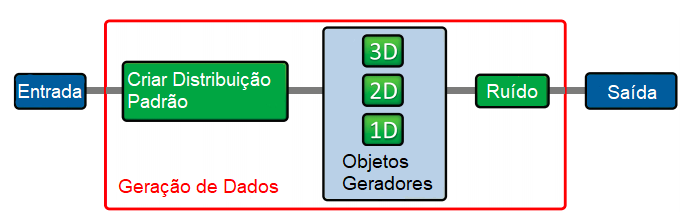
\includegraphics[width=\linewidth]{./figures/TrabalhosRelacionados/Albuquerque10.png}
		\caption{Visão Geral de geração de dados.}
		\label{fig:albuquerque}
	\end{figure}
	\subsubsection{\emph{SketchPadN-D: WYDIWYG Sculpting and Editing in High-Dimensional Space}}
	Wang et al. \cite{BingWang2013} apresentou uma aplicação cujo principal diferencial é a capacidade de modelar, através de desenho, o comportamento das dimensões do conjunto de dados sintéticos. A priori, o usuário pode iniciar o processo de geração através do zero, de um conjunto de dados já existente, ou um conjunto de dados aleatório. A partir disso, o usuário visualiza os dados no gráfico - que pode ser as coordenadas paralelas ou o \emph{scatterplot} - e pode modificá-lo através de cliques e arrastos. Por conseguinte, os dados podem ser gerados e isto também serve como retroalimentação do sistema. Na figura \ref{fig:sketchpad} é possível visualizar a visão geral do funcionamento do SketchPad.
	\begin{figure}[h!]
		\centering
		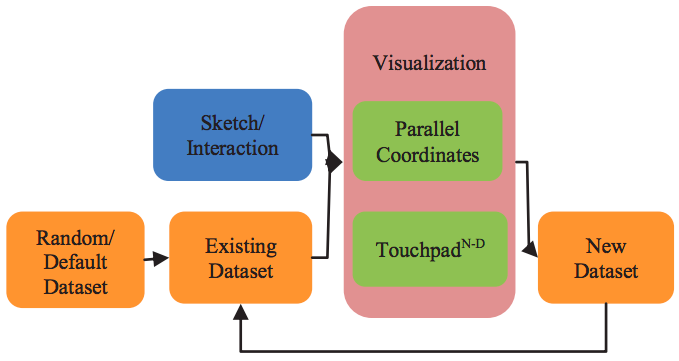
\includegraphics[width=\linewidth]{./figures/TrabalhosRelacionados/Wang11.png}
		\caption{Visão Geral de geração de dados do Sketchpad.}
		\label{fig:sketchpad}
	\end{figure}
	\subsubsection{\emph{Synthetic Data Generator for Classification Rules Learning}}
	Liu \cite{Liu2016} criou um gerador de dados sintéticos a partir de avaliação de regras de aprendizagem. O sistema funciona criando regras de aprendizagem - usando algoritmos de árvore de decisão como o ID3 - baseado em dados de entrada contruindo correlações entre os dados. Na figura \ref{fig:liu} é possível visualizar uma árvore de decisão. Durante a leitura do conjunto de dados de entrada é feita a árvore de decisão e, concomitantemente, são geradas as regras de aprendizagem. Essas regras são utilizadas para gerar amostras de dados sintéticos.
	\begin{figure}[h!]
		\centering
		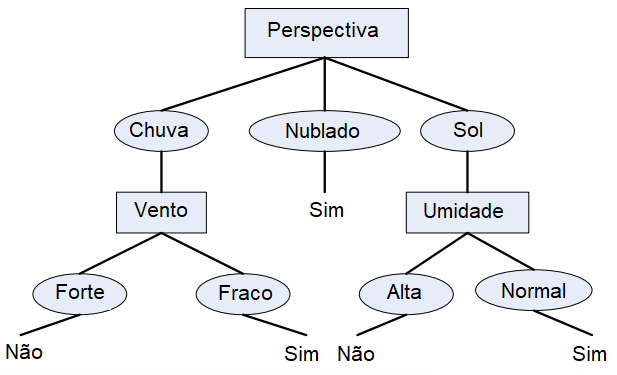
\includegraphics[width=\linewidth]{./figures/TrabalhosRelacionados/Liu13.png}
		\caption{Exemplo de árvore de decisão para jogar tennis criado a partir de regras encontradas em um conjunto de dados.}
		\label{fig:liu}
	\end{figure}
	\subsubsection{\emph{A prototype of synthetic data generator}}
	Garcia e Millán \cite{Garcia2011} criaram um sistema par gerar dados sintéticos pensado para desenvolvedores que buscam testar de forma eficiente e exaustiva a sua aplicação. Esses dados pode ser configurados (ver figura \ref{fig:garcia}) de acordo com as preferências do usuário. As dimensões de dados seguem alguns padrões como a partir de fontes externas (Arquivos, Bibliotecas, Base de dados) Sequencial, Constante, Funcional, Intervalo ou Lista de valores. 
	\begin{figure}[h!]
		\centering
		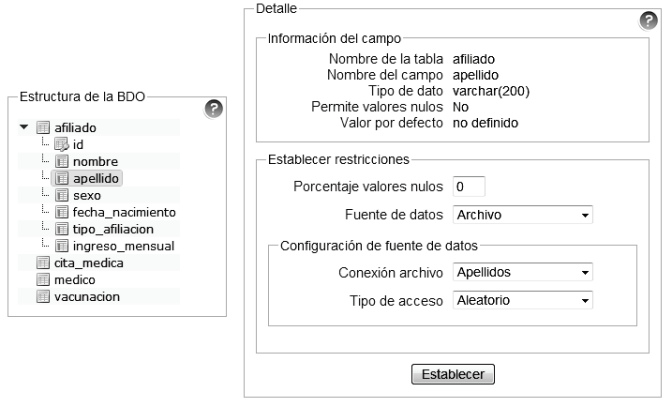
\includegraphics[width=\linewidth]{./figures/TrabalhosRelacionados/Garcia18.png}
		\caption{Exemplo da interface do usuário para configuração do gerador de dados.}
		\label{fig:garcia}
	\end{figure}
	\subsubsection{\emph{A methodology for synthetic household water consumption data generation}}
	Kofinas et al. \cite{Kofinas2018} criou uma metedologia para gerar dados sintéticos para simular consumo de água. A metodologia é avaliada através de algoritmos de validação - como a visualização dos resultados e fórmulas.
	\par
	Como pode ser visto na figura \ref{fig:kofinas}, a geração dos dados é feita a partir de 2 fases. A fase 1 serve, basicamente, para investigar a distribuição dos dados. Esta fase, primeiramente transforma dados números em séries temporais de 30 segundos. Em alguns casos, não há registro, para isso, é criada uma tabela de incidentes e posteriormente uma probabilidade de existência de registro para que seja encontrada as classes usadas para construção do histograma de Pearson \cite{dean2009descriptive}, por fim, são comparadas funções de distribuição com a atual com o fim de encontrar a que mais se aproxima.
	\par
	Para a fase 2 cuida da geração de dados sintéticos propriamente. Basicamente, o sistema utiliza a distribuição criada na fase um para gerar os dados para 24h, respeitando as características diferenciadas para dias de semana e finais de semana.
	\begin{figure}[h!]
		\centering
		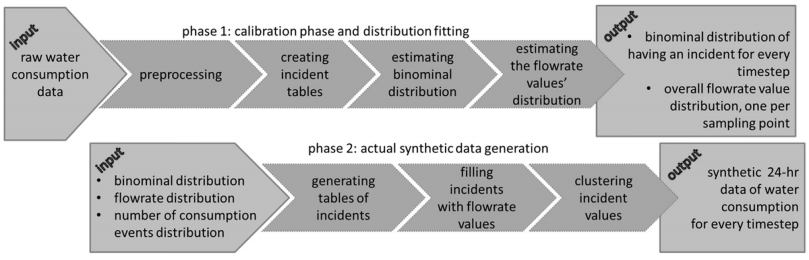
\includegraphics[width=\linewidth]{./figures/TrabalhosRelacionados/Kofinas21.png}
		\caption{Fluxo de passos para geração dos dados sintéticos.}
		\label{fig:kofinas}
	\end{figure}

	\subsubsection{DTM Data Generator}
	DTM Data Generator \cite{DTMDataGenerator} é uma plataforma de geração de dados sintéticos que existe de 1998.
	Esta possui suporte para geração de dados em arquivos, em banco de dados, também para \emph{Big Data}.
	Possui suporte multiplataforma, através do modo \emph{multiplatform runtime}, contudo é limitado quando comparado à versão Windows, o qual suporta a versão para servidor também.
	É válido destacar que é um software essencialmente pago, isto é, existem versões gratuitas - demonstrações, para ser mais exato - mas limitadas.
	Além disso, há categorias de versões pagas, que vão desde limitações de geração (Standart - Professional) à vantagens mais técnicas (Professional - Entrerprise).
	\par
	O DTM Data Generator possui uma vasta coleção de funcionalidades, as quais liberadas de acordo com as versões pagas.
	Adotando a versão mais cara, a lista de \emph{features} é composta por geração de dados em JSON, XML, CSV ou geração por separador customizado.
	Também permite gerar dados por arquivo DSN (Database Source Name), gerar dados por linha de comando, e gerar um arquivo SQL para não seja necessário conexão com banco de dados.
	\par
	É possível gerar cerca de 9.2 sextilhões de registros por \emph{rule}, modos de atualizar dados existentes (adicionar, substituir e \emph{Data Scrambling}), e suporte para bibliotecas de dados realistas.
	A plataforma disponibiliza entrada de dados através de SQL, XML, JSON, pela WEB através de HTTP ou FTP, XLSM, arquivos de texto e scripts em Python.
	Também é possível visualizar e testar os dados gerados, bem como gerá-los nos principais arquivos de texto (TSV, CSV, "DSV", JSON, XML) e banco de dados. (MS SQL Server, Oracle, DB2, MySQL, PostgreSQL, Informix, Sybase, SQLite e Firebird) 
	\par
	Há uma suíte de produtos relacionados fornecidos pela DTM soft. 
	Além do gerador de dados, 
		há o gerador de dados XML para teste de aplicação (DTM Test XML Generator);
		um gerador de planilhas Excel (DTM Data Generator for Excel)
		testador exaustivo - teste de estresse - de banco de dados (DTM DB Stress);
		Bem como editor, visualizador (DTM Data Editor), comparador e sincronizador de banco de dados (DTM Data Comparer) entre outros. 
	\begin{figure}[h!]
		\centering
		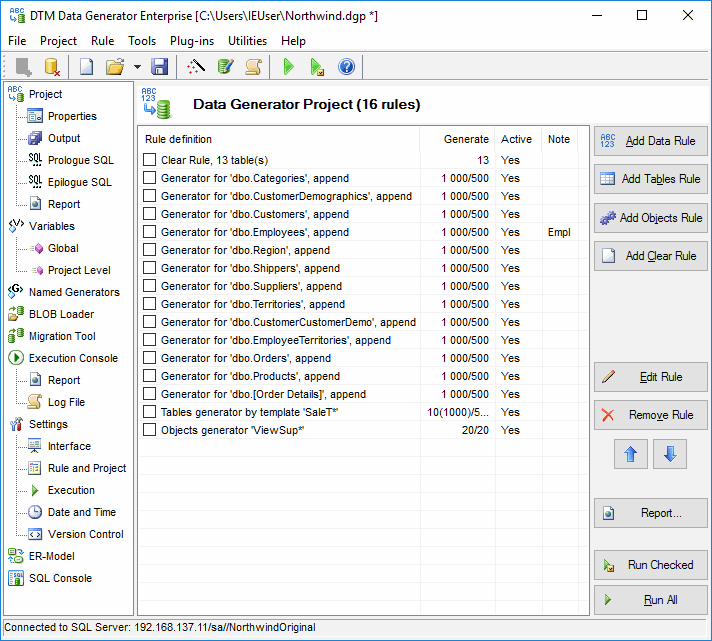
\includegraphics[width=\linewidth]{./figures/TrabalhosRelacionados/DTMDataGenerator.png}
		\caption{Usando o DTM Data Generator. Fonte: DTM Data Generator}
		\label{fig:DTMDG}
	\end{figure}
	\subsubsection{Red Gate SQL Data Generator}
	O SQL Data Generator \cite{RedgateSQLDataGenerator} é um software que compõe uma suíte de ferramentas (chamada de SQL Toolbelt) da Red Gate.
	O software é exclusivo para o ecossistema Windows, com suporte do Windows 7 ao 10, à versão para servidores do Windows, ao SQL Server (2008 ao 2017), .NET e Oracle.
	Este produto é distribuido através de licenças pagas e vitalícias, com atualizações gratuitas e, no mínimo 1 ano de suporte gratuito.
	Vale ressaltar que é possível testar o produto por 14 dias gratuitamente.
	\par
	O SQL Toolbelt tem funcionalidades bem delimitadas e a função do Data Generator é popular um banco de dados. 
	A população acontece ao escolher, primeiramente, uma tabela do banco.
	A partir disso, escolhe-se um gerador para cada coluna da tabela.
	Um gerador tem classificação fortemente baseada na realidade, isto é, possui geradores como palavras relacionadas à compras, pagamentos, pessoas (primeiro e último nome), dado geográficos e afins.
	Contudo, também disponibiliza a geração a partir de expressões regulares \emph{Regex generator} e scripts de python.
	Por se tratar de banco de dados, também há checagem e tratamento de \emph{constraints}, \emph{Foreign keys} e \emph{Dependencies}.
	O SQL Data Generator também permite lidar com arquivos XML, quer seja para geração de valores XML, como utilizar como dados de entrada, além de mesclá-los com o \emph{Regex generator}.
	\par
	Quanto ao SQL Toolbelt oferecido pela Red Gate, ele conta com 2 modalidades, o completo com 14 programas e o \emph{essentials} com 10.
	Entre os mais relevantes, pode-se citar o \emph{SQL Data Compare}, \emph{SQL Data Generator}, \emph{SQL Test}, \emph{SQL Backup Pro} e \emph{SQL Scripts Manager}.
	\begin{figure}[h]
		\centering
		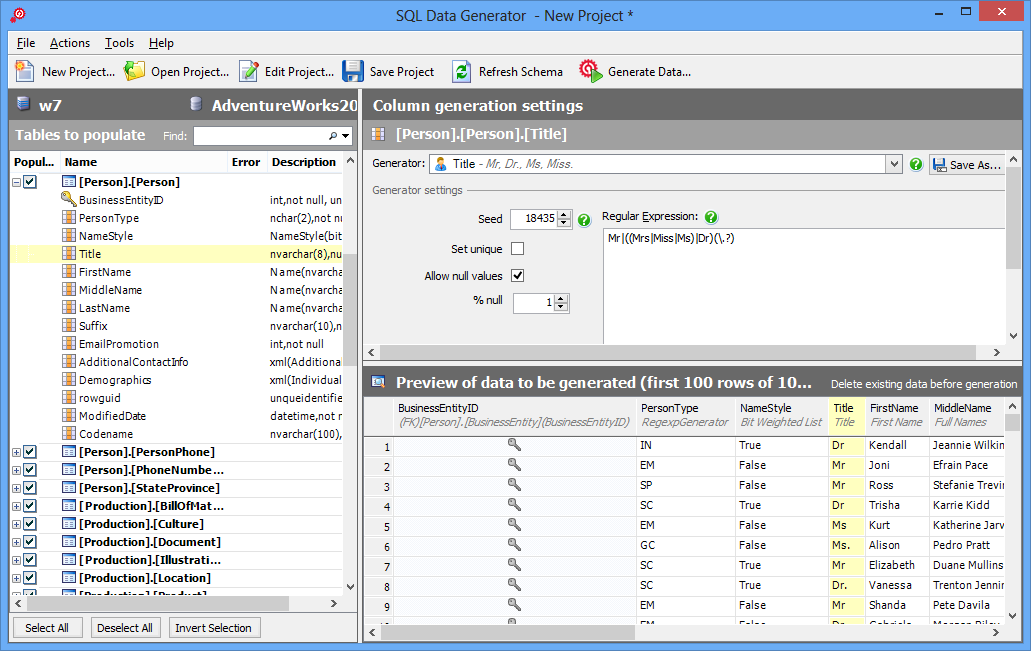
\includegraphics[width=\linewidth]{./figures/TrabalhosRelacionados/sql-data-generator.png}
		\caption{Usando o Redgate SQL Data Generator. Fonte: Red Gate SQL Data Generator.}
		\label{fig:RedgateSQLDG}
	\end{figure}
	\subsubsection{Visual Studio (Premium) Data Generator}
	Microsoft Visual Studio \cite{VSDataGenerator} é um pacote de programas da Microsoft para desenvolvimento de \emph{software}. 
	Este é composto por 4 versões (\emph{Express}, \emph{Professional}, \emph{Premium}, \emph{Ultimate}), e a opção de gerar dados para teste está disponível a partir da versão \emph{Premium}.
	O foco é permitir que verique o comportamento do banco de dados, sem relacioná-los com os dados da aplicação em produção.
	\par
	Para gerar os dados de teste, deve-se utilizar os geradores de dados (\emph{Data Generators}), que são correlacionados às tabelas do banco de dados.
		Os geradores podem ser dos mais primitivos (Binários, Inteiros, Data, \emph{Float}), como de Imagem, Dinheiro, Expressão Regular, Categórico entre outros.
	Também é disponibilizado um Plano de Geração de Dados (\emph{Data Generation Plan}), feito em XML, que contém informações do banco de dados, o tipo de dados de cada gerador e a quantidade de dados para ser gerado. 
	Este plano serve basicamente para reutilização da lógica de teste.
	\begin{figure}[h]
		\centering
		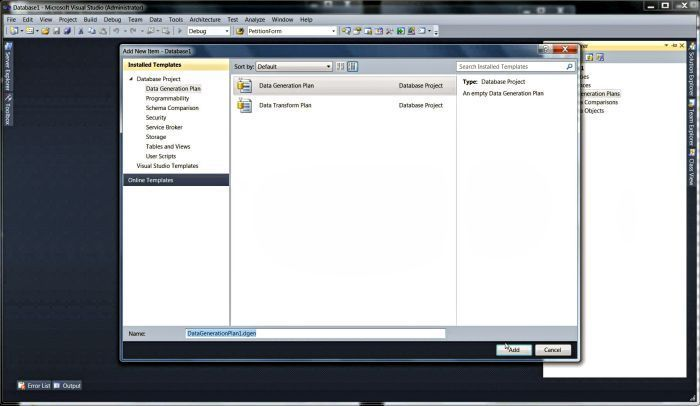
\includegraphics[width=\linewidth]{./figures/TrabalhosRelacionados/Visual-Studio.jpg}
		\caption{Usando o Microsoft Visual Studio. Fonte: anranik.}
		\label{fig:VSDG}
	\end{figure}
	\subsubsection{dbForge Test Data Generator}
	Test Data Generator \cite{forgeDBDataGenerator} é uma ferramenta GUI (\emph{Graphical User Interface}) pela dbForge para gerar dados de teste para banco de dados SQL desde 1997.
	O software possui mais de 200 geradores predifinidos e configuráveis os quais permitem a geração de dados mais inteligentes, isto é, mais próximos da realidade, como nomes, localização, dados de saúde e afins.
	Quanto à compatibilidade, este é exclusivo do ecossistema Windows, com suporte à versão 7 ao 10, do Windows Server 2008 ao 2019 e ao SQL Server Azure, 2008 ao 2017.
	Além da GUI, também há o suporte para geração de dados a partir da linha de comando.
	O produto é distribuido sob licenças pagas e vitalícias, porém, com suporte ao cliente com tempo limitado e com 30 dias gratuitos para avaliação.
	\par
	Para usar o dbForge Test Data Generator, é preciso fazer uma conexão com banco de dados. 
	A partir disso, utiliza-se os \emph{Data Generators} para determinar o comportamento dos dados para determinada coluna da tabela selecionada no Banco de dados.
	Os Geradores de dados podem ser do tipo emph{Basics} e emph{Advanced}. 
	Do primeiro tipo, são formas mais próximas dos dados primitivos, como datas, texto \emph{lorem ipsum}, JSON, \emph{ReGex}.
	Já o avançado conta com número de cartão de crédito, aniversário, número de conta bancária internacional, IPv4, \emph{hash} de senhas.  
	A geração de dados resume-se à população de banco de dados, não há uma forma de exportar os dados em arquivos como CSV e JSON.
	\par
	Há um suíte exclusivo para SQL Server, contudo também para Oracle, MySQL, PostgreSQL entre outros.
	Neste suíte, há várias ferramentas que auxiliam na manutenção, mas não, necessariamente, a geração de dados, a exemplode um \emph{previewer}.
	Destes, pode-se citar um comparador de dados, criador de \emph{querys}, um monitor - para supervisão do banco de dados - e afins.
	\begin{figure}[h]
		\centering
		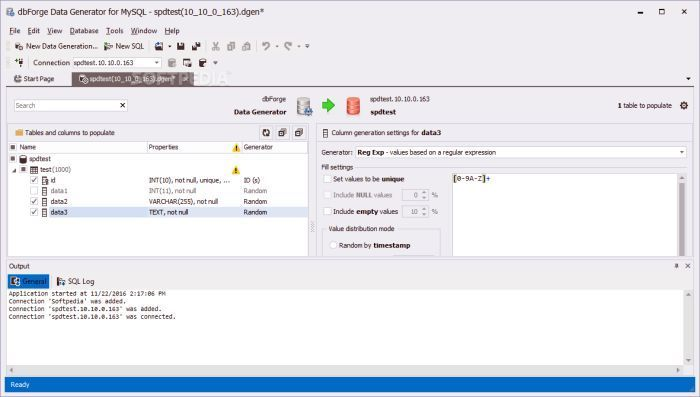
\includegraphics[width=\linewidth]{./figures/TrabalhosRelacionados/dbForge-Test-Data-Generator.jpg}
		\caption{Usando o dbForge Test Data Generator. Fonte: anranik.}
		\label{fig:dbForgeTDG}
	\end{figure}
	\subsubsection{Mockaroo}
	Mockaroo \cite{mockaroo} é um \emph{web site} e \emph{framework} para desenvolver dados de teste.
	Há um total de 143 geradores, sendo a maioria considerados geradores realistas.
	Por ser um site, é possível acessá-lo por qualquer sistema operacional, dependendo apenas de conexão com a internet.
	O produto possui versões gratuita e pagas. - \emph{Free}, \emph{Silver}, \emph{Gold}, \emph{Enterprise} as quais variam no \emph{host}, o qual pode ser do Mockaroo ou privado, máximo de registros por download, velocidade de download e preço.
	\par
	Na tela inicial, é possível escolher o nome da coluna, o tipo de gerador, algumas opções - valores em branco e funções a partir dos dados.
	Ainda nesta tela, encontra-se o botão para \emph{download} dos dados, pré-visualização dos mesmo (mas sem gráficos), algumas configurações como quantidade de linhas, formato dos dados para \emph{download}, botão para clone ou deleção de banco de dados, e importação de dados csv/Excel ou SQL.
	\par
	Outro serviço interessante do Mockaroo é Mockaroo APIs \cite{mockarooAPI}.
	Este consiste em baixar dados programaticamente através de requisições REST (\emph{Representational State Transfer}).
	As requisições podem ser feitas de 2 formas, a \emph{Generate API} - gera os dados através de um banco de dados salvo e os envia pelo corpo de uma requisição - 
	e \emph{Mock APIs} que basicamente, simula um \emph{back-end} como tratamento de parâmetros e simulação de erros. 
	É pensado para desenvolvimento ágil de aplicações \emph{front-end}, isto é, sem perder muito tempo com o \emph{back-end} a priori.
	\begin{figure}[h]
		\centering
		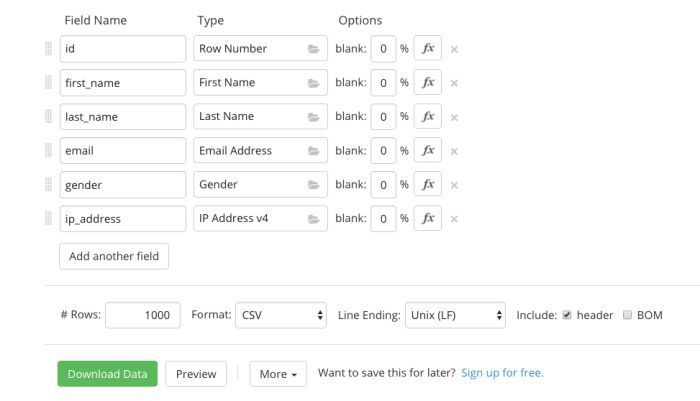
\includegraphics[width=\linewidth]{./figures/TrabalhosRelacionados/mockaroo.jpg}
		\caption{Usando o Mockaroo. Fonte: anranik.}
		\label{fig:mockaroo}
	\end{figure}
	% \subsubsection{ApexSQL Generate}
	% \subsubsection{Datanamic Data Generator MultiDB}
	% \subsubsection{Upscene Advanced Data Generator}
	% \subsubsection{EMS Data Generator}
	% \subsubsection{GEDIS Studio}

	\section{Formato dos dados salvos}
		\subsection{Arquivo}
		%JSON
		JSON \cite{json-rfc-8259} \cite{json-jsonOrg} (Javascript Object Notation, ou em português Notação de Objecto Javacript),lançado em 2002, é uma formatação leve para troca de dados. 
		O uso é facilitado tanto para seres humano quanto para máquina.
		O JSON é um formato de texto que é independente de linguagem, mas foi baseado no objeto provido do Javascript (ECMA-262, 1999).
		\par
		Quanto aos tipos de dados suportados, o JSON \cite{json-rfc-8259} é uma sequência de tokens. 
		Os tipos de tokens aceitos é do tipo \textit{object}, \textit{array}, \textit{string}, \textit{number} e nomes literais como \textit{false}, \textit{true} e \textit{null}.
		\par
		%CSV
		CSV \cite{csv-rfc-4180} (comma-separated values, ou em português Valores Separados por Vírgula) é tipo de texto MIME (Internet Media) \cite{mime-rfc-2048} que utiliza a encodificação de caracteres US-ASCII \cite{csv-rfc-7111}.
		Ao longo dos anos, seu uso foi consolidado para exportar dados entre vários softwares de tabelas (Microsoft suíte para Apple Suíte, por exemplo).
		A padronização do CSV demorou a ocorrer e por isso, vários outros estilos surgiram, a exemplo, o uso do CSV com ponto-e-vírgula (;).
		Outros estilos foram criados a ponto de ser chamado de arquivo DSV \cite{dsv}.
		Por conseguinte, outro estilo que teve notoriedade na troca de dados entre bancos de dados ou tabelas de dados foi o TSV \cite{tsv-iana}.
		A idea é similar ao CSV, porém é utilizado uma tabulação em vez de vírgula.
		
		%\subsection{Banco de Dados}
		\subsection{Web Service}
		\cite{webService-W3C}
		Um Web service é definido como um software sistema criado para suportar interoperabilidade entre máquinas através da rede computadores. Também possui uma interface descrita em um formato processável por máquinas (WSDL) e um protocolo para comunicação (SOAP). \cite{webService-W3C}
		Essa era a arquitetura utilizada em 2004. Atualmente é predominante o uso de REST que em vez de exportar serviços como o SOAP, exporta os dados em si e não necessita do WSDL. \cite{soapVSrest}
		
	% ---
\chapter{Arquitetura do projeto}\label{cap_trabalho_academico}
% ---

%-- TODO: 
		%Inserir metodologia do teste de IHC
			%Vai ser um teste de usabilidade.
		%Inserir os Casos de Uso
		%Inserir as ferramentas utilizadas
	\section{Casos de uso do sistema}
	\section{Ferramentas utilizadas}

% ---
\chapter{Protótipo}
% ---
	Este capítulo é dedicado em explicar mais sobre o prótótipo, seu fluxo de funcionamento, funcionalidades, mais detalhes sobre a interface do usuário entre outros.
	De modo geral, o protótipo é chamado de Blocks Data Generator e visa ser um gerador de dados sintéticos baseado em modelos de dados.
	Assim, o usuário pode manipular um ou mais modelos e cada modelo pode conter N dimensões, que por sua vez podem conter M geradores de dados encadeados.
	Os geradores de dados podem gerar dados numéricos, categóricos, temporais etc (haverá uma seção específica para geradores) e o resultado de um gerador pode servir de entrada para outro gerador através de operadores.
	Os operadores podem ou não aplicar uma operação matemática (soma, subtração, divisão, multiplicação) ao resultado do gerador anterior - a leitura de anterior e posterior é da esquerda para a direita, respectivamente.
	Junto com os operadores, também há outras propriedades que variam de acordo com o gerador (ver seção de Tipos de Geradores de Dados).
	\par
	Ainda na modelagem das dimensões, é possível modificar seu nome, verificar o tipo do dado gerado pelo gerador, o ID e se está disponível para geração e visualização.
	Essa disponibilidade (chamado de \emph{display}) foi feita para o caso de haver um modelo em que nem todas as dimensões sejam necessárias em determinado momento, mas também não queira perdê-las.
	Adicionalmente, é possível copiar e colar dimensões através de atalhos no teclado, bem como adicionar ou excluir dimensões, esta por só meio de um botão.
	\par
	Também é disponibilizado um pré-visualizador de dados com apenas um gráfico - o coordenadas paralelas -, cujo volume de dados é independente do volume de dados para ser gerado, colorido e interativo.
	Além do \emph{preview}, há uma integralização com um visualizador de dados mais elaborado e com mais opções de visualização.
	Outrossim, há um botão específico para gerar os dados em arquivos JSON, CSV, TSV ou por de requisições HTTP do tipo GET (\emph{Web Service}).
	Vale ressaltar que quantidade de dados gerados, pré-visualizados, formato dos dados gerados e se contém a legenda dos dados no arquivo final é configurável em ambiente especializado, assim como para o \emph{Web Service}.
	\par
	% Melhorar a imagem do workflow do Blocks e explicá-la aqui.
	\section{Tipos de Geradores de Dados}
		% TODO: colocar as fórmulas na seção de fórmulas (perguntar para o professor antes)
		\subsection{Sequencial}
		Os geradores da categoria Sequencial geram valores encadeados dado um padrão.
		É possível gerar o próprio padrão a partir do gerador \emph{Custom Sequence}, o qual você determina um valor Inicial (\emph{Begin}), o valor Intervalar (\emph{Step}), isto é, o qual vai ser incrementado ou decrementado dado uma Sentencia (\emph{sentence}) customizada.
		\par
		Contudo, já são predefinidos alguns geradores como 
			o \emph{constant}, o qual define um valor único de geração;
			o \emph{counter}, funciona como um contador, onde-se é definido o valor Inicial e o Intervalar;
			o \emph{Fixed Time Generator} gera um intevalo de tempo, onde-se define o valor inicial (\emph{init}), Intervalar e a máscara (\emph{mask}), isto é, como o tempo deve ser formatado;
			o \emph{Sinusoidal Sequence} gera de acordo com a função senoidal, que, além do valor Inicial e Intervalar, há o 'a' de Amplitude, 'b' de frequência ângular e 'c' para representar a fase da onda.

		\subsection{Aleatório}
		A categoria aleatória de dados são as que contem mais geradores, pois são mais fáceis de se dissociar da realidade, pelo caráter aleatório, mas também de reaproximar, pelo caráter probabilístico.
		Esta categoria conta com geradores uniformes, isto é, a distribuição dos dados é equalizada;
			Também há um gerador de dados de tempo, parecido com o \emph{Fixed Time Generator} com a diferença que o comportamento é definido pela fórmula de Poisson e que há mais duas configurações: unidade de tempo - a qual pode ser desde milissegundos a anos - e o lambda, advindo da fórmula.
			Há uma distribuição de poisson também, apenas com o lambda;
			É disponibilizado geradores de fórmulas clássicas com a normal (Gaussiana), Bernoulli, e Cauchy com seus devidos parâmetros.
			Além de números, também é possível gerar dados categóricos (\emph{Categorical}), dadas as palavras inicialmente.
			Similarmente há o \emph{Weighted Categorical} que possui valores de probabilidade para cada palavra, e 
			já o \emph{Categorical Quantity}, em vez de probabilidade, define quantas vezes cada palavra deve aparecer.
		\subsection{Funcional}
		A categoria funcional \emph{Function} serve para gerar dados de acordo com outra dimensão chamado de \emph{input}, isto é, facilita a correlação entre dimensões.
		Para dados numéricos, disponibiliza-se as 
			função de primeiro \emph{Linear Function} e 
			segundo \emph{Quadratic Function} grau, 
			exponencial \emph{Exponential Function}, 
			logarítmica \emph{Logarithm Function} e
			a \emph{Piecewise Function}, cuja função é definida por subfunções, e no caso, é possível definir o gerador desejado até um determinado valor chamado de \emph{Intervals} e depois pode-se escolher outro gerador.
		\par
		Para dados categóricos, há a função categórica \emph{Categorical Function} e 
		a \emph{TimeLaps Function} a qual funciona de forma semelhante ao gerador \emph{Piecewise Function}, só que utiliza uma quantidade de tempo como limiar, chamado de \emph{Laps} e também somente geradores de tempo como \emph{input}.
		\subsection{Acessórios}
		Os geradores da categoria Acessórios (\emph{Acessory}) foram pensados especialmente para serem concatenados com outros geradores, com o fim auxiliá-los.
		Entre os geradores acessórios, pode-se citar o \emph{Missing Value}, o qual retira alguns dados do conjunto;
			o \emph{Noise Generator} que adiciona dados fora do padrão, conhecido como ruído, com uma determinada probabilidade e intensidade*
			o \emph{Constant Noise Generator} também adiciona ruídos, mas só que é um valor específico com determinada probabilidade de ser adicionado;
			o \emph{Ranger Filter} permite ficar no conjunto de dados apenas os valores que estão entre os valores de início \emph{Begin} e fim \emph{End};
			o \emph{Linear Scale};
			o \emph{No Repeat} retira dados repetidos do conjunto;
			o \emph{MinMax} define quais valores serão os maiores e menores de acordo com os parâmetros dados;
			o \emph{Low-Pass Filter}
			o \emph{Get Extra Value} pega os retornos extras dos geradores que retornam mais que um valor.
		\subsection{Geométrico}
		% Ver Dissertação do Yvan.
		\subsection{Baseado em dados reais}
		Para esta categoria, existe apenas um gerador, chamado como \emph{Real Data Wrapper}.
		Basicamente, ele é criado automaticamente quando o usuário importa um conjunto de dados reais através de um CSV, por exemplo.
		Este gerador recebe tantos valores categóricos como numéricos e essa informação pode ser decidida automaticamente pelo gerador ou ser forçada pelo usuário.
		É possível gerar uma quande superior de dados do que do conjunto de dados real, para isso é feito um tratamento para dados faltantes.
		Esse tratamento é feito através de funções de geração, chamadas de \emph{GenType}.
		\par
		Essas funções pode ser do tipo \emph{Standart}, que é pegar os dados do início ao fim de forma cíclica até chegar ao número desejado de registros.
		Também pode ser do tipo \emph{Reverse} que ao invés do \emph{Standart}, pega os dados do final ao início.
		É disponibilizado o modo aleatório (\emph{Random}), e algumas variações.
		A primeira variação é o \emph{QuartileRandom}, que divide o conjunto de dados em 3 marcos e a probabilidade de se pegar um dado daquele quartil é proporcional ao tamanho do marco.
		A leitura dos Marcos pode ser visualizada na figura \ref{fig:leituraMarco} % TODO: fazer figura do marco.
		A segunda variação é o \emph{AverageRandom} que utiliza o valor da média e da variancia - [Média - Variancia, Média + Variancia] de um conjunto de dados númerico ou utiliza os N valores categóricos mais frequentes com distribuição uniforme.

	\section{Modos de Geração de Dados}

		\subsection{Padrão e \emph{Streaming Data}}
		O protótipo, para uma quantidade limitada de registros e dimensões (5000 e 30 respectivamente) gera os dados agilmente, isto é, bloqueia a interface do usuário, para geração dos dados seja consistente com o modelo.
		O \emph{Streaming Data} foi pensando para o \emph{Big Data}. Então, quando foi passado o limiar da geração padrão dos dados, é criada uma cópia do modelo, para que o usuário seja livre para fazer alterações.
		E para fazer valer essa liberdade, o usuário tem o controle sobre o processo de geração por ver seu progresso e também poder cancelá-lo.
		\subsection{Web Service}
		Quanto ao \emph{Web Service}, este foi pensado para facilitar o teste de aplicação.
		Cada modelo é independente, isto é, podem ser habilitados somente os modelos desejados para distribuição.
		É além da configuração por dentro do \emph{software}, também é possível criar configurações temporárias para cada requisição, sem alterar as configurações o modelo.
		Os parâmetros disponíveis para configuração temporária pela URI são o nome do modelo, o formato dos dados e a quantidade de registro.
		É disponibilizado um aviso ao usuário quando um modelo está distribuindo dados via \emph{Web Service} na aba do modelo.
		Um exemplo de URI para fazer requisição HTTP do tipo GET (http://localhost:8000/?modelid=MODEL_r6w2ffk3.mva&nsample=100&format=csv), nos quais "modelid" é o \emph{ID} do modelo, "nsample" é a quantidade de registros desejado e "format" é o formato dos dados desejado.
	 
	\section{Modos para Visualização de Dados}

		\subsection{Preview}
		\subsection{Sistema de Visualização Externo e Integralizado}

	\section{Estrutura de Interação Humano Computador}

		\subsection{Interface do Usuário}
		\subsection{Mensagens para o usuário}
		\subsection{Atalhos do Teclado}
		\subsection{Ajuda}

% ---
\chapter{Teste}
% ---
\section{Teste de usabilidade do sistema}
% ---
\chapter{Resultados}
% ---
\section{Teste de usabilidade}
% ---
% Conclusão
% ---
\chapter{Conclusão}
% ---

\lipsum[31-33]

% ----------------------------------------------------------
% ELEMENTOS PÓS-TEXTUAIS
% ----------------------------------------------------------
\postextual
% ----------------------------------------------------------

% ----------------------------------------------------------
% Referências bibliográficas
% ----------------------------------------------------------
\bibliography{abntex2-modelo-references}

\end{document}
